\chapter{Background} \label{chap_2}
\ \\
This chapter will provide all the necessary background information and techniques employed in this thesis.
We will start by explaining the concept of \textit{fuzz testing}, with an in-depth analysis of how it works, the main components of a fuzzing session and the different approaches available.
Follows an introduction on software sanitizers, highlighting their relevance in the context of fuzzing.
Then, we provide a short definition on open-source software, the main challenges faced during its development and its connection with fuzzing in the modern era.
Concludes a thorough description of the modern automated testing infrastructures analyzed by this work, detailing their inner working and shortcomings.





\section{Fuzz Testing}

\matteo{Same thing as before about automated testing; automated testing is just a way of saying that the testing is done autonomously (i.e. there is no person behind a screen doing stuff). It doesn't say anything about the involved technique itself (it might be fuzzing, it might be symbolic execution, it might be a monkey pressing random keys etc...)}

One of the most popular approaches to testing a program is \textit{automated testing}, which involves the use of a software separate from the one being tested to control its execution flow and analyze the results obtained, comparing the actual results with the expected ones. It is particularly useful to formalize repetitive tasks into automated operations with high scalability and fast execution times, although manual assessment is still required to ensure the correctness of the operations performed. 

Among automated testing techniques, \textit{fuzz testing} (or \textit{fuzzing}) became increasingly popular and widely used due to its ability to trigger crashes, assertions, memory leaks and undefined behavior. This allows developers to test their programs for so called "corner-cases", meaning situations hard or complex to reproduce when the program is being properly used, that could lead to unexpected and/or unwanted behavior exploitable by malicious people and therefore should be handled properly. It also allows for great flexibility, as this technique can be applied to an entire binary or smaller portions of code, introducing specific testing functions.

We mainly define 3 types of fuzz testing:
\begin{itemize}
    \item \textbf{application fuzzing:} used for UI elements (such as buttons, input fields) or command-line programs, tests may include high-frequency inputs, providing random/invalid content and inputs exceeding the expected size
    \item \textbf{protocol fuzzing:} used to test the behavior of network elements and servers when invalid messages are sent over a chosen protocol, useful to ensure that such content is not misinterpreted and potentially executed as commands
    \item  \textbf{file format fuzzing:} used for programs that accept "structured inputs", i.e. files that have a precise and standard format (like .doc, .jpg), whose structure and content are altered to trigger unwanted behavior
\end{itemize}

This work focused on the third methodology.

\matteo{Here you say that "interesting behaviors" are crashes, then you say that "interesting behaviors" are used to detect coverage. Let's be clear: an "interesting input" might be defined as an input that produces new coverage. That input is going to be mutated further to hopefully get even more coverage and so on. Then, some input trigger crashes: these crashes are reported to the user, but those input are not going to be mutated further.}

The main concept of fuzzing revolves around testing a program on many (seemingly) random inputs over several \textit{fuzzing sessions}, each time discovering a bit more about the structure of the program, and then use this knowledge to create new testcases that attempt to trigger previously unseen execution paths and bugs: when an interesting behavior is observed (i.e. crash, assertion, bugs, ...), the related input is reported to the user and saved for future operations, described in the following paragraphs. 
Each fuzzing session usually takes several hours or days to produce meaningful results; however, because this technique is mostly based on randomness, it also means that results may vastly differ between sessions, even across tests using the same configuration and resources. For this reason, multiple sessions are necessary before a conclusion regarding the safety of the program can be reached.

To determine whether or not a particular testcase resulted in interesting behavior, one of the most popular techniques to analyze its impact is \textit{code coverage}: this metric represents a percentage that defines how much of the source code has been executed during a single fuzzing session, with the assumption that a high value means that most of the code has already been explored and there is a lower chance of having undetected bugs.

This is usually done by creating a "Control Flow Graph" (CFG) of the program, i.e. a representation in graph notation of all paths available during a single execution flow, and measuring: how many nodes (basic blocks) and edges (jumps) were traversed, the number of functions triggered and the branches activated during conditional statements.
Therefore, we define \textit{interesting input} to be any testcase that increases the code coverage achieved and/or triggers a bug during its execution, and it will also be used as reference during the generation of new testcases.






\newpage
\subsection{What is a fuzzer}  \label{fuzzers}
A \textit{fuzzer} is the tool performing fuzz testing, taking as inputs the program being tested and a set of testcases that will be used during the fuzzing session. It is responsible for executing the program against all the provided inputs, analyze each execution and produce new and useful testcases for future fuzzing session.


In general, a fuzzer is composed by the following key elements. \cite{afl_docs}

\textbf{Observer.}\ \ \ Provides information observed during the execution of a program to the fuzzer. Such information may be relatively simple, like the total running time for a test and its output, to more advanced ones, like the maximum depth of the stack. They are usually not preserved across many execution, unless an "interesting input" is encountered, in which case they are relayed to other nodes to improve future fuzzing sessions. 

\textbf{Executor.}\ \ \ Responsible for defining how the program will be executed and the arguments passed on each run. The input for a single test is provided either by writing it in some specific memory location or passed as argument to a so called "harness function", although each fuzzer has its own implementation of this element. Given this, we briefly mention few standard functionalities that compose this element. The \textit{InProcessExecutor} runs the "harness function" and provides crash detection. The \textit{ForkServerExecutor} is responsible for spawning different child processes to fuzz. The \textit{TimeoutExecutor} wraps and installs a timeout for another running executor.

\textbf{Feedback.}\ \ \ Classifies the result of a single execution and determines if the initial input is "interesting" or not analyzing the information received from the observers and the updated coverage map. It's also possible to define several of these elements, each one with its own objective (crashes, timeouts, new execution flows discovered), and combine them in boolean expression to collect more fine-grained results.

\textbf{Input.}\ \ \ Data taken from an external source and provided to the tested program to observe its behavior, usually in the form of bytes arrays. The first fuzzing session takes a set of inputs that is defined and provided by the developer itself, while future fuzzing session will also rely on previously discovered "interesting inputs". 

\textbf{Testcase.}\ \ \ Defined as an input and a set of related metadata, like ID, description and expected results.

\textbf{Corpus.}\ \ \ Location where testcases are stored, usually disk or memory. An example of input corpus may be composed by several testcases with the same properties, like crashing the program under a specific situation. An example of output corpus may be composed by all the testcases that are considered "interesting".



\newpage
Fuzzers can be then categorized using the 3 following characteristics.

\textbf{Input generation.}\ \ \  During each fuzzing session, one of the most important operations performed by the fuzzer is the generation of new testcases, with the objective of diversifying and increasing the effectiveness of the corpora that will be used on future fuzzing sessions: more specifically, an effective fuzzer should be capable of generating inputs "valid enough" so that they are not rejected from the program's parsers, but also "invalid enough" to potentially trigger corner cases. Given this, we  distinguish between \textit{mutation-based} and \textit{generation-based} fuzzers. The \textit{mutation-based fuzzers} require an initial seed of inputs as reference, and the generation of new inputs is performed by applying "mutators" on the provided seeds: these operations range from flipping/adding/removing bits (or bytes), performing mathematical operations and sometimes even completely randomizing its content. Finally, these mutations are usually mixed forming sequences to increase randomness. The \textit{generation-based fuzzers}, instead, rely on a good source of randomness to generate new inputs from scratch, and for this reason they do not depend on the existence of a good initial corpus nor on its quality, although they require more starting time before the tests become effective.

\textbf{Input's structure awareness.}\ \ \ Another information useful to the fuzzer, although not always available, is the "input model", i.e. the correct structure that a file must have when testing programs that follow rigorous standards. However, not all of them provide this feature, and for this reason we define \textit{smart} and \textit{dumb} fuzzers.
A \textit{smart mutation fuzzer} might leverage this knowledge to switch between different types of inputs, while a \textit{dumb mutation fuzzer} can only rely on the structure of the "interesting inputs" and apply limited random mutations, usually resulting in a much lower proportion of valid inputs being generated.
A \textit{smart generation fuzzer} uses this information to avoid wasting resources on generating inputs that are too random to be accepted, as the \textit{dumb generation fuzzer} attempts to generate new inputs without any reference, oftentimes putting more stress on the program's parser rather than the program itself due to the overwhelmingly high number of invalid inputs generated in the first phases.

\textbf{Program's structure awareness.}\ \ \  Fuzzers may be accompanied by program analysis' techniques to increase the efficiency and effectiveness of the tests. A \textit{black-box fuzzer} is completely unaware of the program's structure, therefore assumes the program as a simple machine that takes a random input and generates an according output: this approach is relatively fast, can be easily parallelized and has good scalability, however it will most likely find only bugs that do not require particular conditions to be met to be triggered, also called "surface bugs". A \textit{white-box fuzzer} employs program analysis' techniques to systematically explore and reach critical program locations through meticulously crafted inputs, allowing you to discover bugs that could be potentially hidden deep in the program: while this approach is arguably the most effective one, it implies that bugs related to unknown aspects of the program can be easily missed, and the time used to analyze the program as well as generating such specialized input exponentially increases with the program's complexity.
A \textit{gray-box fuzzer} attempts to find a balance between efficiency and effectiveness by integrating the best aspects of both approaches: using a minimal amount of knowledge over the program's structure to achieve a sufficient degree of code coverage such that the results obtained are satisfactory.




\newpage

\matteo{We used AFL++, not AFL. Maybe you can say that modern fuzzers come from a solution that represented a breakthrough in the fuzzing research (AFL), then say something about, and finally say that this was 10-15 years ago (check it maybe?) and since then other (more precise) solutions have been proposed; AFL++ is one of those and is actually considered the sate-of-the-art solution for fuzzing.}

\matteo{btw, you did not fuzz in this thesis; as far as we know the testcases might be generated with who knows what fuzzers.}

Given all this information, this thesis focused on performing \textit{file format gray-box testing} using the current state-of-the-art fuzzer called \textit{American Fuzzy Lop} (also known as \textit{AFL} \cite{AFL}), defined as a "dumb mutation-based fuzzer". Among the many results achieved by this tool, there are two honorable mentions. In September 2014, AFL discovered "Shellshock" \cite{shellshock} (also known as "Bashdoor"), a family of security bugs affecting the Unix Bash shell that allowed malicious users to execute arbitrary commands without confirmation. In April 2015, AFL discovered the famous "Heartbleed" \cite{heartbleed} bug in OpenSSL, which allowed malicious users to decipher the otherwise encrypted communications used by the TLS protocol. 


\subsection{Fuzzing session (or "Fuzzing session, metrics and bug triage?")}

\matteo{Most of the things you say here explain how fuzzing works better than you explained at the start of 2.1; maybe you can expand that with this information and remove this subsection.}

A \textit{fuzzing session} defines the process of testing a program using a fuzzing tool.
Assuming the program has been properly compiled using the chosen fuzzer, the first step is to simply start the fuzzing session and let the fuzzer execute the program on many different testcases. After some time, when either the initial corpus has been exhausted (mutation-based) or the fuzzer learned what is an acceptable inputs (generation-based), it starts applying random operations to generate new testcases. 

During each execution, code coverage and unexpected behaviors are tracked, so that all testcases that increases any of these statistics will be regarded as "interesting inputs" and saved in a separate queue. In this context, the fuzzer has to be sensible enough to distinguish between crashing and non-crashing inputs without having full knowledge over the program tested, and therefore \textit{sanitizers} are used to "instrument" the source code and inject assertions that make the program crash when a particular kind of failure is detected. Section \ref{sanitizers} explains this concept more thoroughly.

At the end of each fuzzing session, the user is presented with three results: a collection of statistics regarding the coverage achieved and bugs found, a list of inputs that caused crashes along with some metadata (testcase ID, bug type, memory state, etc...), and a set of "interesting inputs" that can be used in future fuzzing sessions to provide the fuzzer with even more information about the structure of a good input that explored the deepest parts of the program. 
The statistics provided may be useful to understand how effective this particular fuzzing session was with respect to the previous ones, if the initial corpus needs to be refined and whether the changes applied to the code have been fruitful or not.
The new set of "interesting inputs" is then added to the existing initial corpus, which in turn is \textit{pruned}: this process removes any duplicates and inputs that trigger the same execution flow or bugs, which is crucial to ensure that the size of the corpus does not explode over time.
Finally, the developer has to analyze all the inputs that caused a bug and perform \textit{bug triage}: execute each input individually to observe its output, determine which kind of error occurred and why, fix the bug entirely (if possible) or at least patch the problem, and ensure that the bug does not occur in future fuzzing sessions by including the triggering input(s) in the set used for the tests.

All these steps are repeated across many different fuzzing sessions, sometimes even changing the scope of the tests to increase code coverage or stressing the program with many buggy inputs, each time making the program more secure against vulnerabilities and more robust to extraneous inputs. 




\newpage
\section{Sanitizers} \label{sanitizers}
A \textit{code sanitizer} is a tool used to detect bugs in a program during both compilation and runtime, with different sanitizers specializing in detecting different kinds of bugs: misuse of addresses, stack- and heap-overflows, use of uninitialized memory and leaks as well as undefined behavior.

They are added to a program through "instrumentation", which refers to modifying either the source code or the binary code to introduce some additional functionalities and references that can be used by other tools to perform code analysis, logging or profiling. Although code sanitizers should be a standard practice in the development cycle of a program, unfortunately this is not the case as introducing these tools not only requires extensive tests to check for potential errors, but also because they do not always interact very well with shared libraries or other external dependencies. It is also extremely important to mention that these bug detection tools are not meant to be linked against production executables, as their runtime was not developed with security-sensitive constraints and may compromise the security of the released product. \cite{asan_docs}\cite{msan_docs}\cite{ubsan_docs}

A \textit{compile sanitizer} is a tool that performs instrumentation at compile-time, meaning that it introduces functions and libraries that will be then added and compiled together with the original source code, effectively altering its default behavior. Their advantages are twofold: they are able to achieve full coverage and provide warnings and errors during the compilation process, since the analysis is performed directly on the source code and includes all possible paths, and they are also able to detect errors during the execution of the program, although obviously limited by the single execution flow analyzed. However, these sanitizers introduce a non-trivial overhead both in terms of increased compile time, execution time and memory usage, which may cause problems when it comes to managing computing resources.

A \textit{binary sanitizer} is a dynamic binary instrumentation (DBI) framework that performs "Just-in-Time" (JIT) compilation to introduce additional instructions and analysis callback during the execution of a program, effectively without modifying the original code, and they often rely on dynamic binary analysis (DBA) tools to analyze programs at run-time at the level of the machine code. Also these sanitizers are dependent on the input given and the resulting execution flow analyzed, therefore they are not capable of achieving full code coverage. Moreover, this analysis requires attaching another external process to instrument the original one, which usually causes massive slowdowns and sometimes might even break the original's code functionality.  

This work focused on using several compile sanitizers developed by Google \cite{san_repo} as part of its tool suit provided to open-source developers, along with a popular binary sanitizer \cite{valgrind_web} to perform a cross-check on the results produced by the compile sanitizers, as these tools have been proven to be particularly effective when combined with fuzzing due to their ability to trigger bugs.




\newpage
\subsection{ASan and LSan}
The \textit{Address Sanitizer} \cite{serebryany2012addresssanitizer} is a memory error detection tool for C/C++ that helps developers to find and fix any out-of-bounds accesses to heap, stack and global objects, use-after-free bugs and provides protection against stack-based and heap-based overflow, making it one of the most popular and effective sanitizers.

When allocating bytes for a buffer and performing an access beyond such boundaries, a program will usually crash with an "out-of-bounds exception", but it could also happen that it is valid to access information in the unallocated address, in which case the program will crash unexpectedly and make it difficult for the developer to understand the problem. Moreover, if such addresses are not properly freed, they could leave a so called "dangling pointer", and thinking that this memory location still holds valid data (maybe even confidential one) implies serious security issues.
If an attacker discovers a program with such vulnerabilities, he could use them to crash the application, corrupt or retrieve sensitive data, or even perform a "remote code execution" attack by inserting some malicious code via this buffer overrun and causing the program to jump and execute that particular memory location, creating an attack vector where anything is possible. 

To prevent this, the sanitizer uses a shadow memory to map the memory regions allocated by the application and record whether each byte of such areas can be safely accessed by load/store operations. Each memory region is assigned a shadow counterpart, containing metadata about its size and the offset range that can be used to safely access it, while any attempt to read/write beyond such boundaries will trigger a sanitizer error, as shown by the figure below:

\begin{figure}[h]
\centering
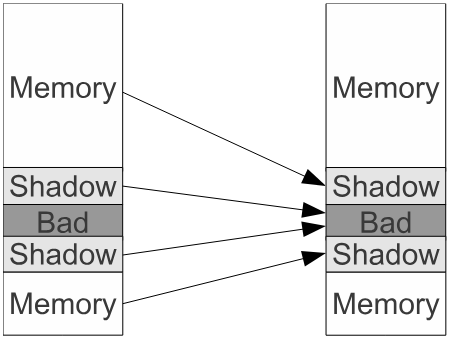
\includegraphics[scale=0.6]{foto/shadow_memory.png}
\caption{Memory mapping of ASan \cite{serebryany2012addresssanitizer}}
\label{fig:asan_shadow}
\end{figure}

Detection of out-of-bounds accesses to globals and stack objects is done in a similar way, i.e. by creating poisoned memory regions around such objects: \textit{global variables} are poisoned at compile-time and their addresses computed during the application startup, while \textit{stack objects} are poisoned and recorded at run-time.

The management of the shadow memory is done by ASan run-time library, containing specialized implementation of the \verb|malloc| and \verb|free| functions, which allocate extra memory for shadow and poisoned memory zones as well as keeping a FIFO stack of allocated and freed memory regions to detect use-after-free, double-free and invalid-free bugs.

This sanitizer is also provided with another component called \textit{Leak Sanitizer} (or \textit{LSan}), a memory leak detector enabled by default that returns which portions of the program are leaking memory as well as the size leaked, thanks to comprehensive and exhaustive stack traces. A memory leak is a condition where a program fails to release memory that is no longer needed due to developers' negligence or software error, effectively reducing the amount of memory available by the machine, and this will inevitably lead to performance degradation (trashing). Although this component may seem very helpful, it usually generate huge logs especially when having complex programs that heavily rely on external libraries, which oftentimes do not perform clean releases of the objects used.

Finally, ASan adds a slight overhead, increasing execution times by an average 170\% and memory usage by 3.4x. \cite{serebryany2012addresssanitizer}





\subsection{MSan}
The \textit{Memory Sanitizer} \cite{stepanov2015memorysanitizer} is a memory reads detector for C/C++ that helps developers to find and fix use-of-uninitialized-memory (UUM) bugs, which are considered to be quite tricky as they do not necessarily occur in every execution and could be triggered by any operation performed by the program. This is because the C/C++ languages are defined "memory-unsafe" due to the fact that the management of the memory is left to the developer, who is responsible for correctly allocating, using and freeing any memory region that is accessed by the program: in fact, unless specified, any new allocation operation performed by these languages creates uninitialized stack and heap objects. Such vulnerabilities may not only be exploited to alter the execution flow and inject malicious code, but also to leak information about a program's internal stake, such as the content of the stack or heap.

A UUM bugs usually originates from any operation that loads a value from an uninitialized memory region, resulting in an \textit{undefined value} being returned, and operations like conditional branch, syscall and pointer dereference are most likely to trigger them. This sanitizer works by using a shadow memory to map each bit of application memory and encode its state (0 initialized, 1 otherwise): all newly allocated memory is poisoned, i.e. the corresponding shadow memory is initialized to \verb|0xFF|, and "shadow propagation" operations are performed to safely copy an uninitialized variable to different memory regions as well as safely perform simple logic and arithmetic operations on them without occurring in errors.

\begin{figure}[h]
\centering
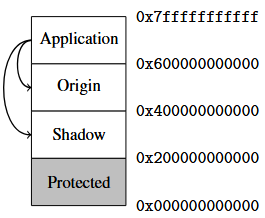
\includegraphics[scale=0.8]{foto/shadow_memory_2.png}
\caption{Memory mapping of MSan \cite{stepanov2015memorysanitizer}}
\label{fig:msan_shadow}
\end{figure}

Given that UUM bugs are notoriously hard to reproduce and debug, MSan provides the "origin-tracking-mode" to obtain more comprehensive and descriptive stack-traces. If necessary, there is also the "advanced-origin-tracking-mode", which records the entire stack and all operations that happen between the allocation and load of uninitialized variables, but its usability is still discussed due to the huge amounts of memory it requires.

The management of the shadow memory is done by MSan run-time library, that maps the "shadow" and (optional) "origin" areas and marks as uninitialized any new allocated regions as well as the deallocated ones. To update the shadow region, a large subset of the standard \verb|libc| functions are intercepted.

Fixing these bugs generally requires little to none effort, but many developers avoid this sanitizer due to the huge slowdown that it introduces. In fact, MSan increases execution times by an average 300\% and memory usage by 2x on short programs, values that rapidly worsen with complex programs. \cite{stepanov2015memorysanitizer}





\subsection{UBSan}
The \textit{Undefined Behavior Sanitizer} \cite{ubsan_docs} is a fast undefined-behavior detector for C/C++, that helps developers to find and fix undefined-behavior (UB) bugs. The C language specification allows developers to perform many complex and (sometimes) unreasonable operations on the assumption that they know what they are doing, and this leads to the compiler making arbitrary decisions when the code does not conform to some expected values: for example, an array indexed with an out-of-bound value will not always crash the program if said memory location contains valid content that belongs to the program, while performing a conversion between two data types of different sizes will result in unpredictable loss of data due to rounding operations. This means that different compilers will handle such situations differently and produce unexpected results each time they are executed, all without taking into account that the hardware used and the level of optimization chosen will also affect these results.

Common operations that may lead to undefined behaviors are: array subscription out of bounds, overflows/underflows of numerical types due to mathematical or logical operations, shifts of numerical values, dereferenced, misaligned or null pointers and invalid conversions between data types. Although this list is not exhaustive of all possible scenarios, it is apparent that most of the problems mentioned could be fixed with negligible effort and avoided altogether by applying appropriate coding standards.  

This sanitizer works similarly and sometimes overlaps with ASan, putting protected regions around buffers and inserting correctness-checking functions after all mathematical, logical and implicit/explicit cast operations. By default, due to its simplistic nature, the tool does not print stack-traces and uses a minimal run-time library, although the "print-stacktrace-mode" option can be enabled to obtain more comprehensive results.

To conclude, UBSan adds a trivial overhead, increasing execution times by an average 120\% and memory usage by 2x. \cite{ubsan_docs}



\subsection{Valgrind}

\matteo{Valgrind is a DBI, not a sanitizer. On top of valgrind, memcheck was developed. memcheck is a tool that performs binary sanitization (I.e. it checks some property at run-time).}

\matteo{When you describe something done from others, I suggest you to open the main page of their site and read the description they give; start from there, especially if you are not familiar with the topic. For example, the site for valgrind says: "Valgrind is an instrumentation framework for building dynamic analysis tools. There are Valgrind tools that can automatically detect many memory management and threading bugs, and profile your programs in detail. You can also use Valgrind to build new tools."}

The Valgrind tool is a binary-level sanitizer, more specifically a Dynamic Binary Instrumentation (DBI) framework that performs code analysis at run-time, capable of achieving full coverage of user-mode code. \cite{Valgrind_1} \cite{Valgrind_2} It allows code profiling and memory analysis, with similar functionality to ASan and MSan, and provides several tools that can be used to debug the executed program.

The tool relies on dynamic binary recompilation to load the client program into the \textit{Valgrind Core} and (re)compile the client's machine code in small blocks using a "Just-In-Time" (JIT) approach, producing a so-called "Intermediate Representation" (IR) which is then instrumented with analysis code. This translated code is then stored in a code cache, so that it can be rerun when necessary avoiding this overhead. It is also capable of monitoring the CPU registers during the program execution by taking control of the real CPU and (conceptually) running the client program on a simulated one, and the concept of "shadow memory" is used to analyze and protect both memory and CPU registers.

In this work, Valgrind was mainly used as a substitute of MSan to detect UUM bugs when analyzing projects that relied heavily on external libraries: this is because, of the compile sanitizers mentioned above, MSan is the only one that requires all libraries linked to the executable to be rebuilt with this sanitizer in order to get meaningful results. However, this process turned out to be too cumbersome and beyond the scope of this work, also because most projects use statically linked libraries rather than compiling them from scratch.

While this tool is very popular and widely used, it also suffers from a major limitation due to its design choice, which is that it is a single-threaded program: this means that its execution cannot be parallelized and the entire program and its analysis run on a single CPU core and kernel thread. In fact, Valgrind applies an average slowdown of 4x by default, value that can range from 10x up to 100x for CPU-bound programs when other analysis tools are introduced. \cite{Valgrind_1}





\newpage
\section{Open-Source Software}
The \textbf{Open-Source Software (OSS)} is a computer software developed in a collaborative and public manner, released under a particular license that allows other users to freely use, study, modify and distribute the software and its source code for any purpose: this allows many users to actively participate in the development of a software by proposing changes and new improvements.
To be eligible as an open-source software, the license's distribution terms must comply with several criteria \cite{osd}: the main concept is to let anyone easily download your program and access its the source code, allowing them also to modify and redistribute the project without additional fees as long as the original code is appropriately credited. 

Given all this, one could argue that making all this information publicly available poses a real threat to security: history has shown us many times that, given enough time and resources, releasing the source code of a program will result in malicious users discovering bugs and vulnerabilities that could have potentially catastrophic consequences.

For this reason, we mention some key aspects that should be considered when approaching open-source software.

\textbf{Development.}\ \ \ Open-source software is usually released under two development branches: a "stable" version, composed by all the functionalities that have been thoroughly tested and work as intended, and a "build" version, that is slightly buggier as it includes proposed changes and new features that have yet to be refined. Releasing the "build" version early not only allows the developers to showcase their work and attract even people, but also provides them with feedback from real users that are willing to run untested versions of their software.

\textbf{User interaction.}\ \ \ Providing full access to the source code means that other users might want to contribute in the program's development and help the developers in improving and refining the product: considering that each user may have different knowledge and programming skills as well as different testing environments, this allows them to test and benchmark the product on a wide range of systems, further increasing the probabilities of finding new and unknown bugs that may be specific to a single OS or architecture.

\textbf{Bug reporting.}\ \ \ Although any user has the rights to mention a bug, error, or mistake in the program or the documentation, it is still up to the developers to ensure the truthfulness of what has been reported and how to tackle it. For example, bugs that are not security-relevant or that may be related to QoL aspects are easily pushed back as secondary problems or simply ignored altogether. Sometimes, if the developer are kind enough to accept your request but do not have time and resources to solve it, they might ask for a proposed fix and cite the user themselves in the next patch notes as a way of thanking them.

\ziosaba{I've rewritten this section to be more concise and straightforward, as I would really like to keep it}


\newpage
\section{Continuous Fuzzing}
\matteo{Introduce Google's role in the description.}
\ziosaba{Google's role as in? the fact that it provides its own infrastructure for fuzzing and how it allows (virtually) any open-source project to enter this campaign?} 
\matteo{Continuous fuzzing is a concept. Then, google implements it through some frameworks. You should introduce the concept, describe it thoroughly and then discuss who does it and how it does it.}

The \textit{Google Open Source Project} \cite{google_oss} is a campaign started in 2004, one of the oldest open-source campaigns in the industry. 

It was initially meant to share Google-developed software under open licenses, with the intention of bringing free technology and information sharing to the public, but it quickly became a program dedicated to improving open-source ecosystems as a whole. 
Thanks to this campaign, many projects became popular and gained worldwide recognition such as Android OS, TensorFlow, the Go programming language, and many more.

\ziosaba{This thesis will focus on two campaigns maintained by Google called \textit{OSS-Fuzz} \cite{ossfuzz_docs} and \textit{FuzzBench} \cite{{fuzzbench_docs}}: the first is a free platform that allows open-source developers to fuzz their programs autonomously relying on the computing resources provided by the Google Cloud service, while the latter allows fuzzer developers to test and improve their tools on real-word benchmarks thanks to automated tests and reports.
More specifically, it revolves around fuzzing some of the projects that have been implemented in these repositories using alternative approaches, trying to discover bugs that will be then securely reported and disclosed to their developers in hope to have them fixed.}

\subsection{ClusterFuzz}
The \textit{ClusterFuzz Project} is a scalable fuzzing infrastructure with the objective of discovering security and stability issues in software, it is the main platform used by Google to test its own products and also the fuzzing back-end for \textit{OSS-Fuzz}.

As of May 2023, it discovered over 25.000 bugs in Google proprietary software (e.g. Chrome) and 36.000 bugs with OSS-Fuzz. \cite{clusterfuzz_docs}
It is based on a highly scalable distributed system of VMs, performing fully automatic bug filing, triage and closing as well as performance reports.
\begin{figure}[h]
\makebox[\textwidth][c]{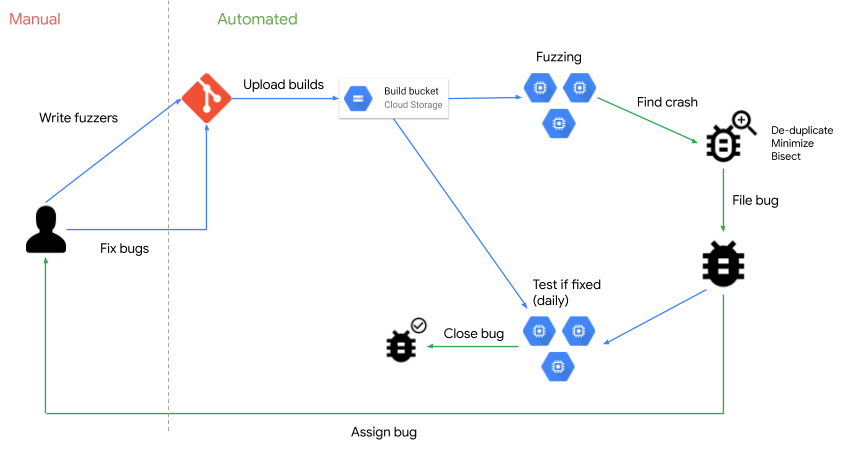
\includegraphics[width=0.665\paperwidth]{foto/clusterfuzz_architecture.png}}
\caption{ClusterFuzz main architecture visualized \cite{clusterfuzz_docs}}
\label{fig:clusterfuzz_architecture}
\end{figure}
\ \\
All operations are performed by two components.
The \textit{App Engine} provides a web interface to the information collected during each fuzzing session, allowing the developers to easily access crashes, results and other information. This is also where tests can be scheduled, which is done via \verb|cron| jobs.
The \textit{Fuzzing Bots Pool} is a cluster of VMs responsible for running the scheduled fuzzing sessions, and they perform the following operations:
\begin{itemize}
    \item \textbf{fuzz:} runs a fuzzing session
    \item \textbf{progression:} checks if a testcase still reproduces or if has been fixed
    \item \textbf{regression:} calculates the revision range in which a crash was introduced
    \item \textbf{minimize:} eliminates duplicate testcases from the input seeds
    \item \textbf{pruning:} minimize a corpus to the smallest size based on coverage information
    \item \textbf{analyze:} runs a manually uploaded testcase against a specific job to see if it crashes
\end{itemize}

\matteo{Same thing as before about paragraphs, these 3 belong together.}

Given that some of this tasks are critical and should be treated as atomic operations, bots can be \textit{preemptible} or \textit{non-preemptible}.

The first refers to a machine that can only run the "fuzz" task as it can be shut down at any moment.

The latter refers to a machine that is not expected to abruptly stop or crash, therefore is capable of running all tasks.
Each VMs performs these operations inside Docker instances, created and provided by the developer using Dockerfiles, that are configured with all the tools and files necessary to correctly build and launch the fuzzing targets.


\subsection{OSS-Fuzz}

\matteo{This section gives lots of practical details, that may or may not be useful, but does not say things that could actually be useful, like how long does a fuzzing session last (6 hours if I'm not mistaken, but check it), what seeds are used (this is kind of important, since we are going to analyze the queues), that the queues are actually saved (and re-used), that there multiple fuzzers etc.}

\matteo{I am not saying this is bad overall, I am just saying that you can improve it significantly by giving more useful information; remember that the people who will read this will most likely know close to nothing about fuzzing, they are much more interested in knowing how fuzzing is deployed here than knowing that there is a script called "build.sh" that performs automatic building.}

The \textit{OSS-Fuzz Project} \cite{ossfuzz_paper} was created in 2016 after the famous "Heartbleed" vulnerability was discovered in OpenSSl, one of the most popular open-source projects at the time for encrypting web traffic, as a response to provide developers with free fuzzing and private alerts services for their open-source projects.
While it was initially intended for languages that are not memory-safe (C/C++), it is now capable to provide support for other popular languages such as Python, Go, Java and Rust.  

As of August 2023, it helped identify and fix over 10.000 vulnerabilities and 36.000 bugs across over 1000 projects. \cite{ossfuzz_docs}.
Projects can be tested using several fuzzing engines (such as LibFuzzer, AFL++, Honggfuzz and Centipede) in combination with Google Sanitizers (ASan, MSan and UBSan), while \textit{ClusterFuzz} acts as the back-end and reporting tool.

\begin{figure}[h]
\makebox[\textwidth][c]{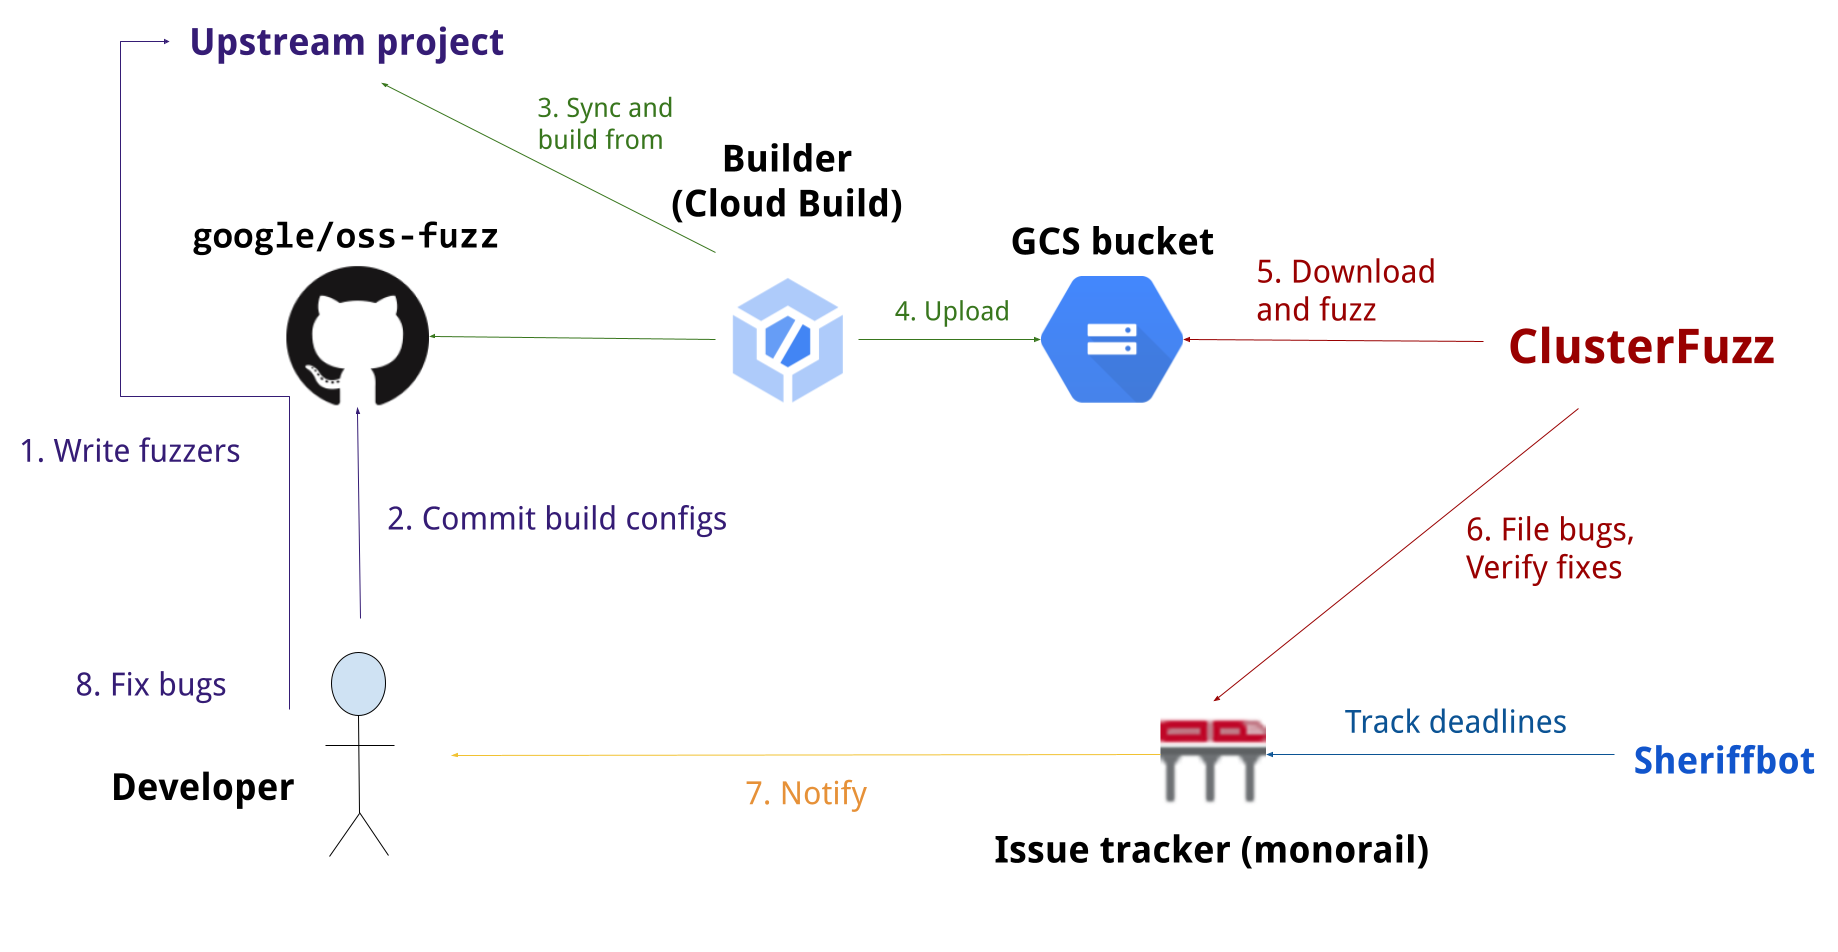
\includegraphics[width=0.65\paperwidth]{foto/oss-fuzz_architecture.png}}
\caption{OSS-Fuzz main architecture visualized \cite{ossfuzz_docs}}
\label{fig:ossfuzz_architecture}
\end{figure}

The architecture is structured as follows:
Initially, the maintainer of an open-source project creates one or more "fuzz targets" that will be integrated with the project's build and test systems. \cite{libfuzzer_docs}

A "fuzz target" is essentially a function that accepts an input, in this case an array of bytes, and perform some operations with these bytes to test a specific API.

Although not all projects are expected to implement and maintain their targets in the same way, developers can refer to a guide of recommendations to increase the efficiency and quality of the automated fuzzing tests performed.
To briefly summarize them, they should:
\begin{itemize}
    \item maintain the source code and targets' build system using some versioning service (like Git)
    \item allow each fuzz target to be compiled with Sanitizers
    \item avoid modular build systems for the fuzz targets (compile all or nothing) and use general-scope compile flags
    \item provide a seed corpus that is regularly updated and extended with new "interesting inputs", also it should have good coverage
    \item provide a dictionary of tokens to instruct the fuzzer on the correct syntax of the inputs, if applicable
    \item periodically check the performances achieved by each fuzz target, meaning their coverage, time spent on execution and solving abrupt errors
\end{itemize}

To be accepted by OSS-Fuzz, a project must be relevant and/or critical to the global IT infrastructure and it must have a significant user base.
To check if your project is eligible for OSS-Fuzz, Google provides a mathematical formula to calculate the "Open-Source Project Criticality Score" \cite{score} in a range between 0 \textit{(least critical)} and 1 \textit{(most critical)}:
\ \\ 

\begin{equation}
    CriticalityScore = \frac{1}{\sum \alpha_i}\  \sum_i \alpha_i \ \frac{\log(1+S_i)}{\log(1+\max(S_i,T_i))}
\end{equation}
where $\alpha_i$ refers to the "weight" of an indicator and $T_i$ its maximum allowed value.

The parameters evaluated are the followings:
\begin{itemize}
    \item \textbf{created-since} ($\alpha_i = 1$, $T_i = 120$): months since the project was created, older projects have higher chances of being widely used or being dependent upon
    \item \textbf{updated-since} ($\alpha_i = -1$, $T_i = 120$): months since the project was last updated, unmaintained projects with no recent commits have higher chance of being less relied upon
    \item \textbf{contributor-count} ($\alpha_i = 2$, $T_i = 5000$): count of commits made by project contributors, different contributors involvement indicates project's importance
    \item \textbf{org-count} ($\alpha_i = 1$, $T_i = 10$): count of distinct organizations contributing to the project, indicates cross-organization dependency
    \item \textbf{commit-frequency} ($\alpha_i = 1$, $T_i = 1000$): average number of commits per week in the last year, code that changes constantly means higher susceptibility to vulnerabilities
    \item \textbf{recent-releases-count} ($\alpha_i = 0.5$, $T_i = 26$): number of releases in the last year, frequent releases indicates user dependency
    \item \textbf{closed-issues-count} ($\alpha_i = 0.5$, $T_i = 5000$): number of issues closed in the last 90 days, indicates contributor involvement and focus on closing user issues
    \item \textbf{updated-issues-count} ($\alpha_i = 0.5$, $T_i = 5000$): number of issues updated in the last 90 days, indicates high contributor involvement
    \item \textbf{comment-frequency} ($\alpha_i = 1$, $T_i = 15$): average number of comments per issue in the last 90 days, indicates  user activity and dependence
    \item \textbf{dependents-count} ($\alpha_i = 2$, $T_i = 500000$): number of project mentions in the commit messages, indicates repository use
\end{itemize}
\ \\
Only projects scoring a value $\geq 0.7$ may be eligible to be integrated in the OSS-Fuzz campaign.


\newpage
Assuming your project satisfies the score requirements, developers issue a "pull request" on the OSS-Fuzz repository providing the following 3 files.
The \textit{project.yaml} configuration file stores project metadata needed by OSS-Fuzz to correctly provide its services, and some of the most commons are:
\begin{itemize}
    \item \textbf{homepage:} url to the project's homepage
    \item \textbf{language:} programming language used to write the project (C, C++, Go, Rust, Python, JVM languages, Swift)
    \item \textbf{primary\_contacts:} list of email addresses that will be automatically CCed on crash reports and fuzzer statistics
    \item \textbf{main\_repo:} path to the source code repository hosting the project
    \item \textbf{vendor\_ccs:} \textit{optional}, list of vendors' email addresses that want access to the bug reports
    \item \textbf{sanitizers:} \textit{optional}, list of sanitizers that are available on the project (address, undefined, memory), if not specified "address" and "undefined" will be used
    \item \textbf{architectures:} \textit{optional}, list of architectures that can build the project (supported only x86\_64 and i386)
    \item \textbf{fuzzing\_engines:} \textit{optional}, list of fuzzing engines available (libfuzzer, afl, honggfuzz and centipede), if not specified "libfuzzer" will be used
    \item \textbf{builds\_per\_day:} \textit{optional}, number of times a project should be built per day, OSS-Fuzz allows up to 4 builds per day and builds once per day by default
\end{itemize}
\ \\
The \textit{Dockerfile} defines a container with all the dependencies and resources needed to build the project and prepare the testing environment.

To avoid having developers create and maintain their own customized Docker containers and create an homogeneous and standard environment, OSS-Fuzz provides several "base images" for each supported language, built on top of Ubuntu 20.04 and with the appropriate compilers and toolchains already installed.

After pulling the most appropriate base image, there are usually several "apt-get" and "git clone" commands related to downloading and installing all the required packages and dependencies needed to correctly build the project.

Finally, the build script and any other fuzzer files are pulled from the project's repository.
The \textit{build.sh:} script, executed inside the Docker container, performs all the operations necessary to build the project and the fuzzing targets that will be tested.

In general, the script should build the project and the fuzz targets using the correct compiler and appropriate compiler flags.

To provide a more flexible and accessible build system, the Docker image provides several environment variables regarding directory locations, compilers and compiling flags, allowing developers to easily re-target scripts with little effort.
On the other end, a bot periodically checks for new requests and validates their content before accepting/rejecting them.



Once the project has been accepted as part of the OSS-Fuzz's infrastructure, a "builder" script follows the provided instructions to build the project's fuzz targets and uploads them to a Google Cloud Service Bucket, a file-hosting service.

This acts as a middle point between OSS-Fuzz and ClusterFuzz, which uses the aforementioned bucket to download all the necessary elements to fuzz the project as well as upload the results achieved.
After a successful fuzzing session, any bug discovered is reported to the OSS-Fuzz issue tracker \cite{ossfuzz_bugtracker}, which uses the metadata sent by ClusterFuzz to create its report. 

Developers have 3 ways of dealing with this situation: they can commit new changes to fix the bug (verified by ClusterFuzz before closing an issue), assign the tag "WontFix" to the bug to notify that it will not be solved, or simply ignore it altogether. 
Finally, OSS-Fuzz follows a strict \textit{bug disclosure guideline}. \cite{bug_disclosure}
When a bug is discovered, an automatic email is generated and sent to all email addresses specified in the project, and an issue is opened on the issue tracker.

This email contains the report created using ClusterFuzz, as well as an estimation of the priority and severity of the bug discovered.
From this moment, the issue will be publicly visible in 90 days or after the fix is released (whichever comes earlier), meaning that anyone will have access to the causing input as well as any other debugging information related to what happened and how to reproduce the bug.

Before the deadline expires, the developers may request a 14-day grace period if the patch is set to be released on a specific day within this extended period, in which case the public disclosure is delayed.
In any case, Google reserves the right to change deadlines forwards or backwards depending on the circumstances and the severity of the findings.

\subsection{FuzzBench}

\matteo{Again, you are providing many practical details, that are neither very interesting nor useful; you say that fuzzers are added through pull requests, but you do not say what benchmarks are being used, in what version (and then you should comment on the choice of an old version -> this is done to provide a fixed version for constant comparison through the year, plus those versions are known to contain bugs), what seeds are used, if queues are re-used (they don't, unlike OSS-Fuzz), what types of experiments can be performed (coverage vs bugs, until last year, now it was changed as you told us)}

\matteo{Lastly, we are finding many bugs in sbft23, so you should probably do a subsubsection on that and say anything interesting in you can find about it, like what subjects were used (I think 5 were public at first but 10 were not public, so that the competition could be performed on subject the authors did not test) and so on. Look for material on the internet, I am providing two links down here in comments}

%https://sbft23.github.io/tools/
%https://storage.googleapis.com/www.fuzzbench.com/reports/experimental/SBFT23/Final-Bug/index.html

The \textit{FuzzBench Project} \cite{fuzzbench_paper} is a free service that provides fuzzers' developers with several real-world benchmark tested at Google scale, comparing the results with other famous fuzzers (such as AFL and LibFuzzer) and allowing them to evaluate their performances thanks to daily reports for further improvements.
\cite{fuzzbench_docs}

\begin{figure}[h]
\makebox[\textwidth][c]{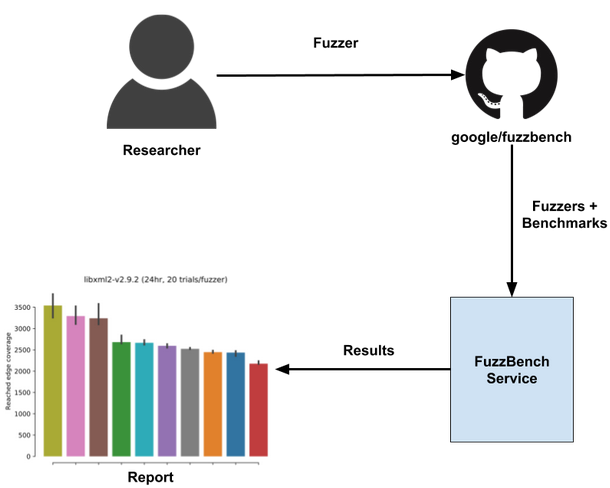
\includegraphics[width=0.68\paperwidth]{foto/fuzzbench_architecture.png}}
\caption{FuzzBench main architecture visualized \cite{fuzzbench_docs}}
\label{fig:fuzzbench_architecture}
\end{figure}

The infrastructure is structured as follows.
Initially, a fuzzer developer integrates its product within FuzzBench using a Dockerfile, containing all the resources necessary to build targets using the fuzzer and also where all benchmarks will be executed.

Similarly to OSS-Fuzz, this process is done via "pull requests", which are automatically revisioned and accepted by bots.
Then, the developers may choose between two testing approaches: standard and OSS-Fuzz.

In the first case, the benchmark is created by the developers themselves, and this requires the definition of fuzz targets, build files and Docker images that will be used to correctly build and link the fuzzer to the targets and run the tests.

In the latter, the developers employ a fuzz target from any OSS-Fuzz project as benchmark, allowing them to test their product on a real-world scenario.
Finally, a report will be created highlighting the strengths and weaknesses of the fuzzer on the various benchmarks, comparing individual and overall results with other integrated fuzzers.